\documentclass[10pt,twocolumn,letterpaper]{article}

\usepackage{cvpr}
\usepackage{times}
\usepackage{epsfig}
\usepackage{graphicx}
\usepackage{amsmath}
\usepackage{xcolor}
\usepackage{listings}
\usepackage{amssymb}
\usepackage{algorithmic}
\usepackage{graphicx}  
\usepackage{multicol}
\usepackage{pdfpages}
\usepackage{pythonhighlight}


% Include other packages here, before hyperref.

% If you comment hyperref and then uncomment it, you should delete
% egpaper.aux before re-running latex.  (Or just hit 'q' on the first latex
% run, let it finish, and you should be clear).
\usepackage[breaklinks=true,bookmarks=false]{hyperref}

\cvprfinalcopy % *** Uncomment this line for the final submission

\def\cvprPaperID{****} % *** Enter the CVPR Paper ID here
\def\httilde{\mbox{\tt\raisebox{-.5ex}{\symbol{126}}}}

% Pages are numbered in submission mode, and unnumbered in camera-ready
%\ifcvprfinal\pagestyle{empty}\fi
\setcounter{page}{1}
\begin{document}

%%%%%%%%% TITLE
\title{\LaTex\ Image Style Conversion using Cycle-Consistent Adversarial Networks}

\author{16341023 Fu-Rong Zhou\\
School of Data and Compute Science\\
Sun Yat-Sen University \\
{\tt\small 543536324@qq.com}
}
% For a paper whose authors are all at the same institution,
% omit the following lines up until the closing ``}''.
% Additional authors and addresses can be added with ``\and'',
% just like the second author.
% To save space, use either the email address or home page, not both
%

\maketitle
%\thispagestyle{empty}

%%%%%%%%% ABSTRACT
\begin{abstract}

   Image style conversion refers to the conversion of image content 
   from one domain to another.This tasks generally require paired 
   pictures with the same content in the both domains as training data.
   Such as pix2pix\cite{pix2pix}, but this pair of training data is difficult to obtain.
   The innovation of CycleGAN is that can migrate picture content from
   the source domain to the target domain without paired training data.
   Paper“Unpaired Image-to-Image Translation using Cycle-Consistent Adversarial Networks”\cite{CycleGAN}
   presents an approach (Cycle-GAN)for learning to translate an image from a source
   domain to a target domain in the absence of paired examples. Quantitative comparisons 
   against prior methods demonstrate the superiority of their approach.
   
\end{abstract}

%%%%%%%%% BODY TEXT
\section{Introduction}

   The original author realized the conversion of image style through CycleGAN: 
   zebra to horse, summer to winter interchange. Can we apply this technology 
   to the automatic conversion of the portrait of a comic character to the costume, 
   and generate a new anime character through the original anime character's avatar and costume, 
   which will greatly reduce the illustrator's design of a new anime character. time.
   
   The core idea of ​​CycleGAN is that if there is an image style converter G that 
   can convert the image of the X domain into the style of the Y  domain, 
   and F can convert the image of the Y domain into the style of the X domain, 
   then G and F should be reciprocal. That is, after the image of the X field is converted to $\hat{Y}$ by G, 
   $\hat{Y}$ should be converted to X by F. 
   Similarly, after the image of the Y field is converted to $\hat{X}$ by F, 
   $\hat{X}$ should be converted to Y by G. 
   That is: F(G(x))=x; G(F(y))=y. 
   To implement this Cycle Consistency, the paper uses a Cycle Consistency Loss\cite{CycleConsistencyLoss}:
   
   L_{cyc}(G,F) = E_{x\sim p_{data}(x)}[\left \| F(G(x)) - x \right \|_{1}]
   
   + E_{y\sim p_{data}(y)}[\left \| G(F(y)) - y \right \|_{1}] \cite{CycleGAN}
   
  
   CycleGAN is a circular structure consisting of two generators and two discriminators.
   X represents the image in X domain and Y represents the image in Y domain. 
   The image in X domain is generated by    generator G in Y domain, 
   and then the original image input in X domain is reconstructed by generator F. 
   The image in Y domain is generated by generator F, 
   and the original image input in Y domain is reconstructed by generator G. 
   Discriminator Dx and Dy play a discriminant role to ensure the style migration of images.
   
   CycleGAN is essentially two mirror symmetrical GANs\cite{GAN}, forming a ring network. 
   Two GANs share two generators with a Discriminator. One-way GAN has two losses, 
   and CycleGAN has four losses.
   As shown in the figure \ref{fig:one} , CycleGAN is actually composed of two discriminators (Dx and Dy) and two generators (G and F), 
   in order to avoid all X being mapped to the same Y,
   in order to avoid this situation, we adopts two generators, which can satisfy the mapping of X $\to$ Y and satisfy The mapping of Y $\to$ X, 
   in fact, is the idea of variational self-encoder VAE, in order to adapt to different input images to produce different output images.
   


\begin{figure*}
\begin{center}
   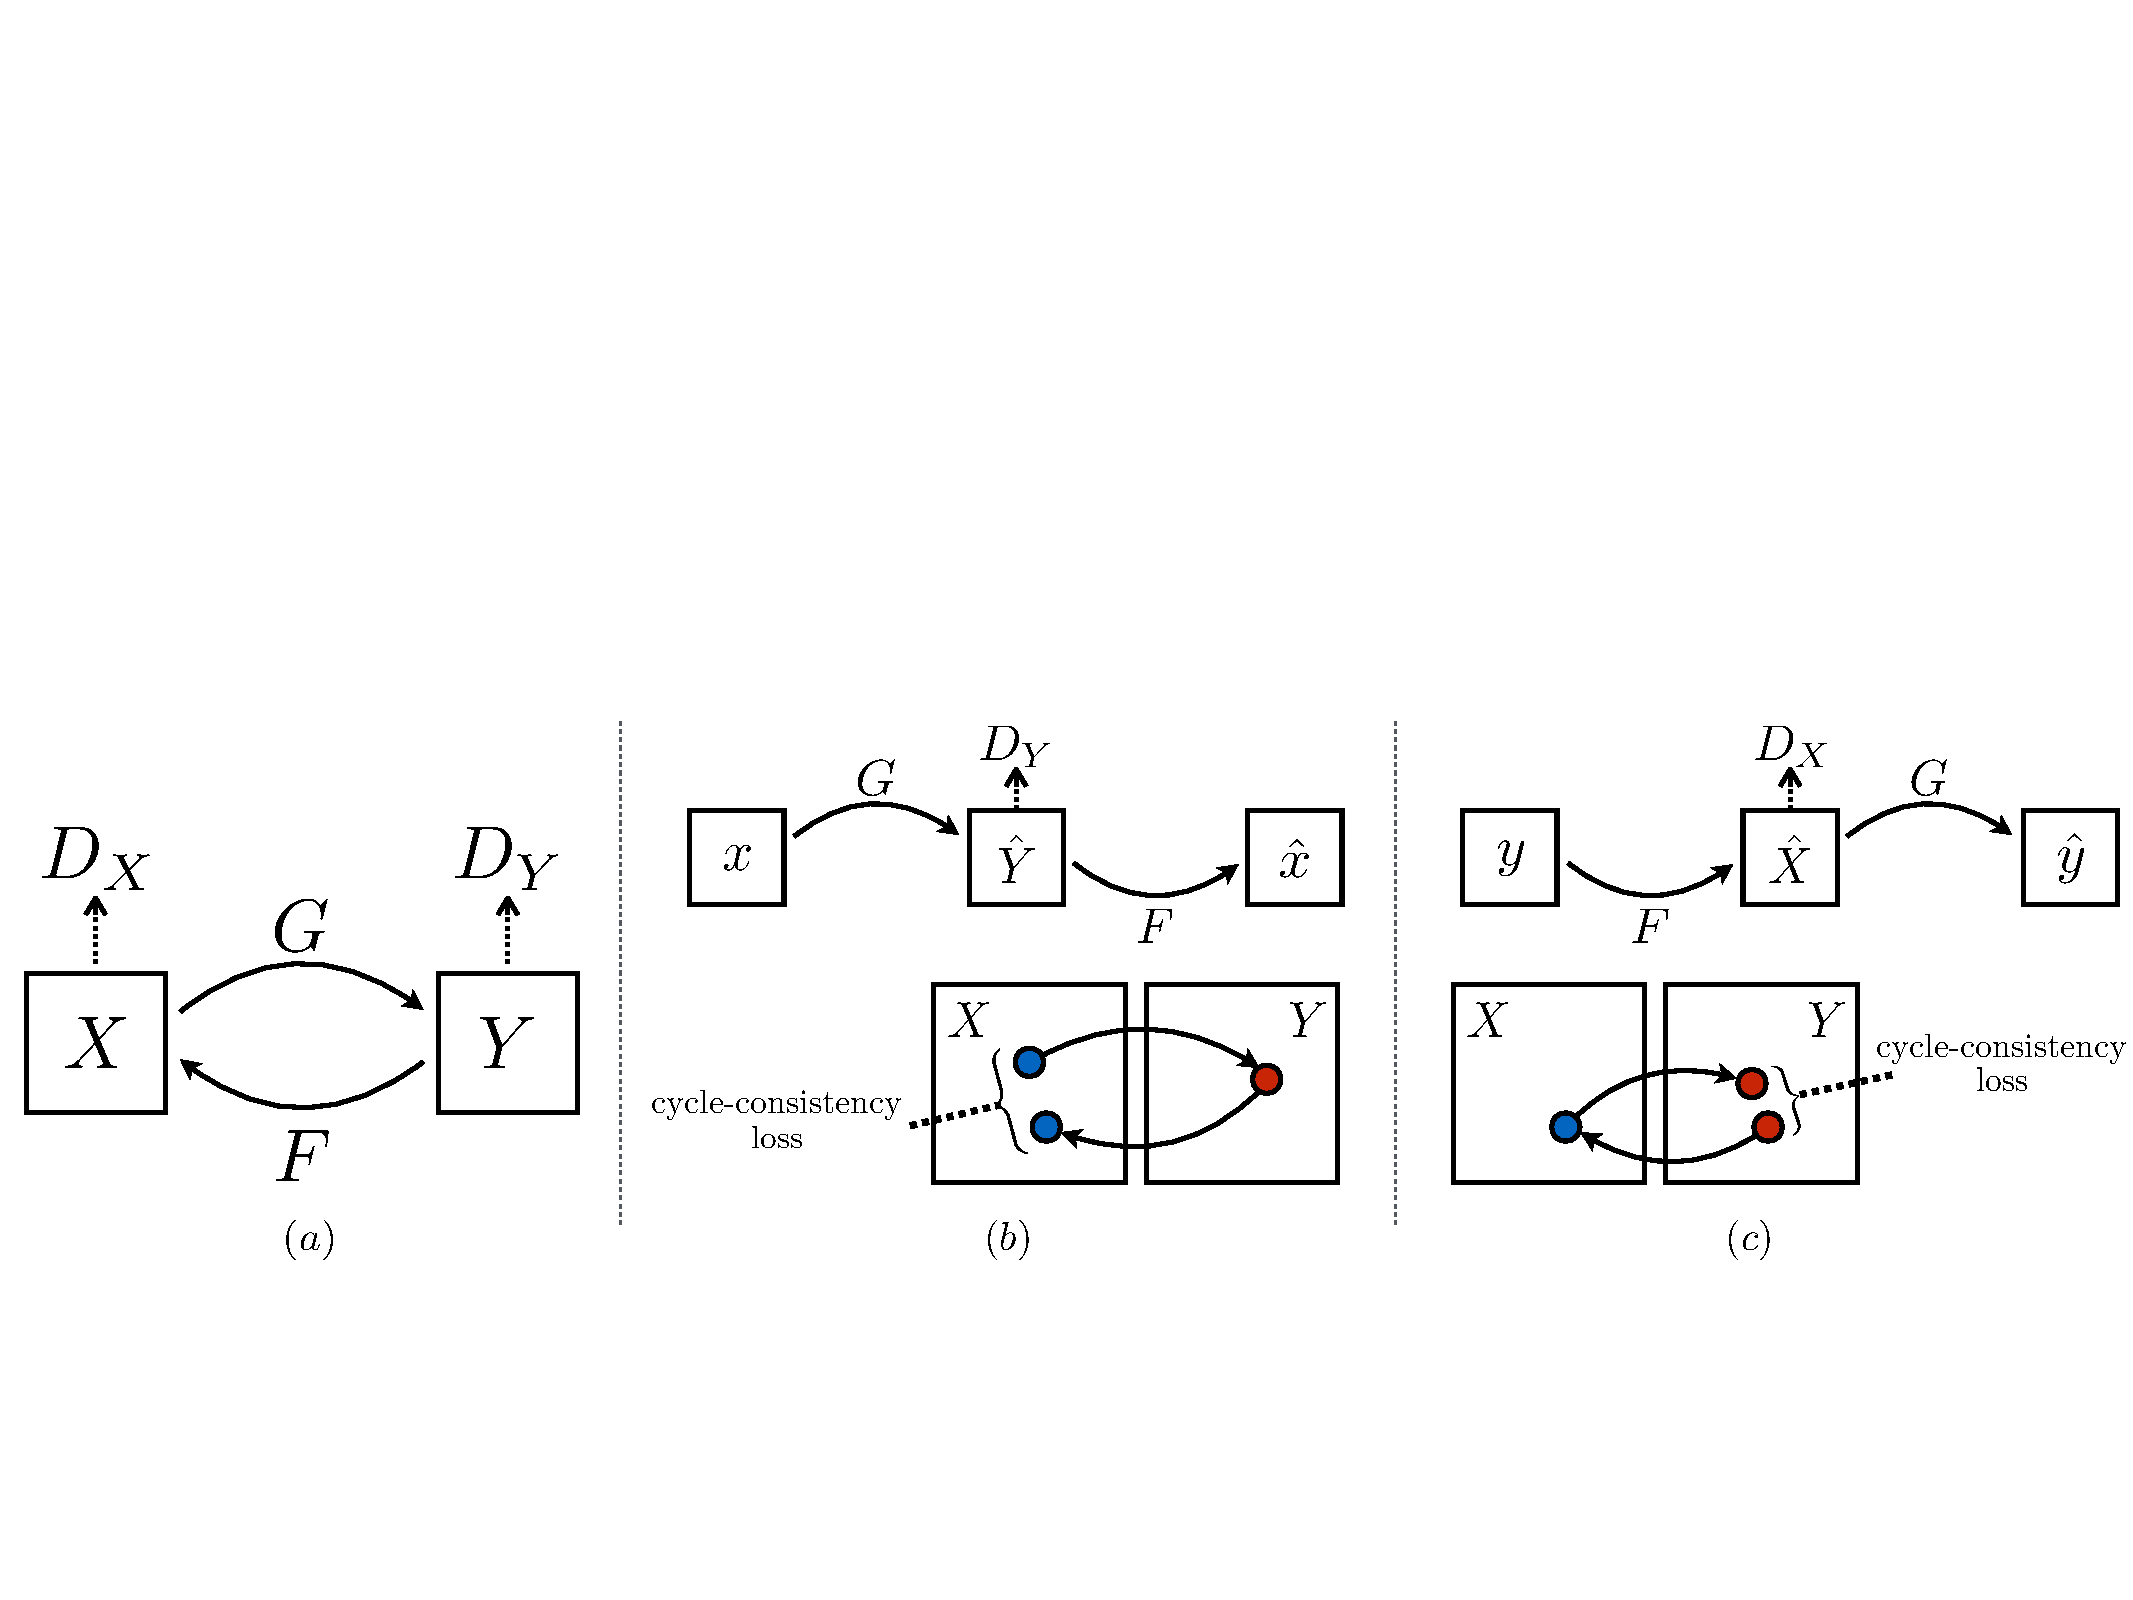
\includegraphics[width=0.9\linewidth]{system_diagram_v2.pdf}
\end{center}
   \caption{CycleGAN is actually an A→B one-way GAN plus a B→A one-way GAN. The two GANs share two generators, each with a discriminator, so adding up to a total of two discriminators and two generators. A one-way GAN has two losses, and CycleGAN adds up to a total of four losses.}
\label{fig:one}
\label{fig:onecl}
\end{figure*}


%-------------------------------------------------------------------------

\subsection{Related work}

As researchers at home and abroad pay more and more attention to image migration,
A series of Cyclegan algorithms have emerged.
In this section, we briefly introduce four related work.
( Generative Adversarial Networks (GANs)、
Image-to-Image Translation、
Unpaired Image-to-Image Translation、
Cycle Consistency )

{\bf Generative Adversarial Networks (GANs)}~\cite{GAN,GAN1}
have achieved impressive results in image generation\cite{imagegen,imagegen1},
image editing \cite{imgaeedi}, 
and representation learning\cite{imagegen1,replearn}.
The key to the success of GAN is 
the concept of confrontational loss, 
which forces the generated image to be 
indistinguishable from the real image in principle.

{\bf Image-to-Image Translatio}:
The idea of image to image conversion 
is to use a non-parametric texture model\cite{texmodel}
 on a single input-output training image pair. 
 The latest method uses the data set of 
 input and output checks to learn the 
 parameter conversion function through CNN\cite{CNN}. 
 Our approach is based on the "pix2pix"\cite{pix2pix} 
 framework of Isola et al\cite{Isola}.
 It uses conditional generation of the network 
 to learn the mapping from input to output images.
 
 {\bf Unpaired Image-to-Image Translation}:
 The similarity function between the predefined inputs 
and outputs that does not depend on any particular task, 
nor does it assume that we assume that the inputs 
and outputs must be in the same low-dimensional 
embedded space. This makes our approach a 
universal solution for many visual and graphical tasks.

{\bf Cycle Consistency:}
In target tracking, language translation, 
3D shape registration and so on. 
There are also applications in CNN. 
A similar loss was introduced to push G and F 
to agree with each other.



\section{technical background}
\subsection{formula :}

Adversarial Loss:For the mapping function G : X → Y and its dis- criminator DY , we express the objective as

\begin{align}
\mathcal{L}_{\text{GAN}}(G,D_Y,X,Y) =  \ \mathbb{E}_{y \sim p_{\text{data}}(y)}[\log D_Y(y)] \nonumber \\
+  \ \mathbb{E}_{x \sim p_{\text{data}}(x)}[\log (1-D_Y(G(x))]
\end{align}

\begin{align}
  \mathcal{L}_{\text{GAN}}(G,D_X,X,Y) =  \ \mathbb{E}_{x \sim p_{\text{data}}(y)}[\log D_X(y)] \nonumber \\
  +  \ \mathbb{E}_{y \sim p_{\text{data}}(x)}[\log (1-D_X(G(x))]
  \end{align}

  Cycle Consistency Loss. The so-called Cycle consistency is to ensure
  
  Forward consistent: x $\to$G(x)$\to$F(G(x))≈x
  
  Backward agreement: y$\to$F(y)$\to$G(F(y))≈y

  We incentivize this behavior using a cycle consistency loss:
 \begin{align}
   \mathcal{L}_{\text{cyc}}(G, F) =  mathbb{E}_{x\sim p_{\text{data}}(x)} [[{F(G(x))-x}]_1] \nonumber \\ 
   + \ \mathbb{E}_{y\sim p_{\text{data}}(y)}[[{G(F(y))-y}]_1]
 \end{align}

 full objective loss function is:
 \begin{align}
  \mathcal{L}(G,F,D_X,D_Y) = \mathcal{L}_{\text{GAN}}(G,D_Y,X,Y) \nonumber \\
  +\ \mathcal{L}_{\text{GAN}}(F,D_X,Y,X) \nonumber \\
  +\  \lambda \mathcal{L}_{\text{cyc}}(G, F)
 \end{align}
 
 
 {\bf Depth generation model :}
 
 
The network architecture of CycleGAN is shown in the figure\ref{fig:1}:

  


\begin{figure}
  \centering
\subfigure[a]{
  \begin{minipage}[b]{0.9\textwidth}
  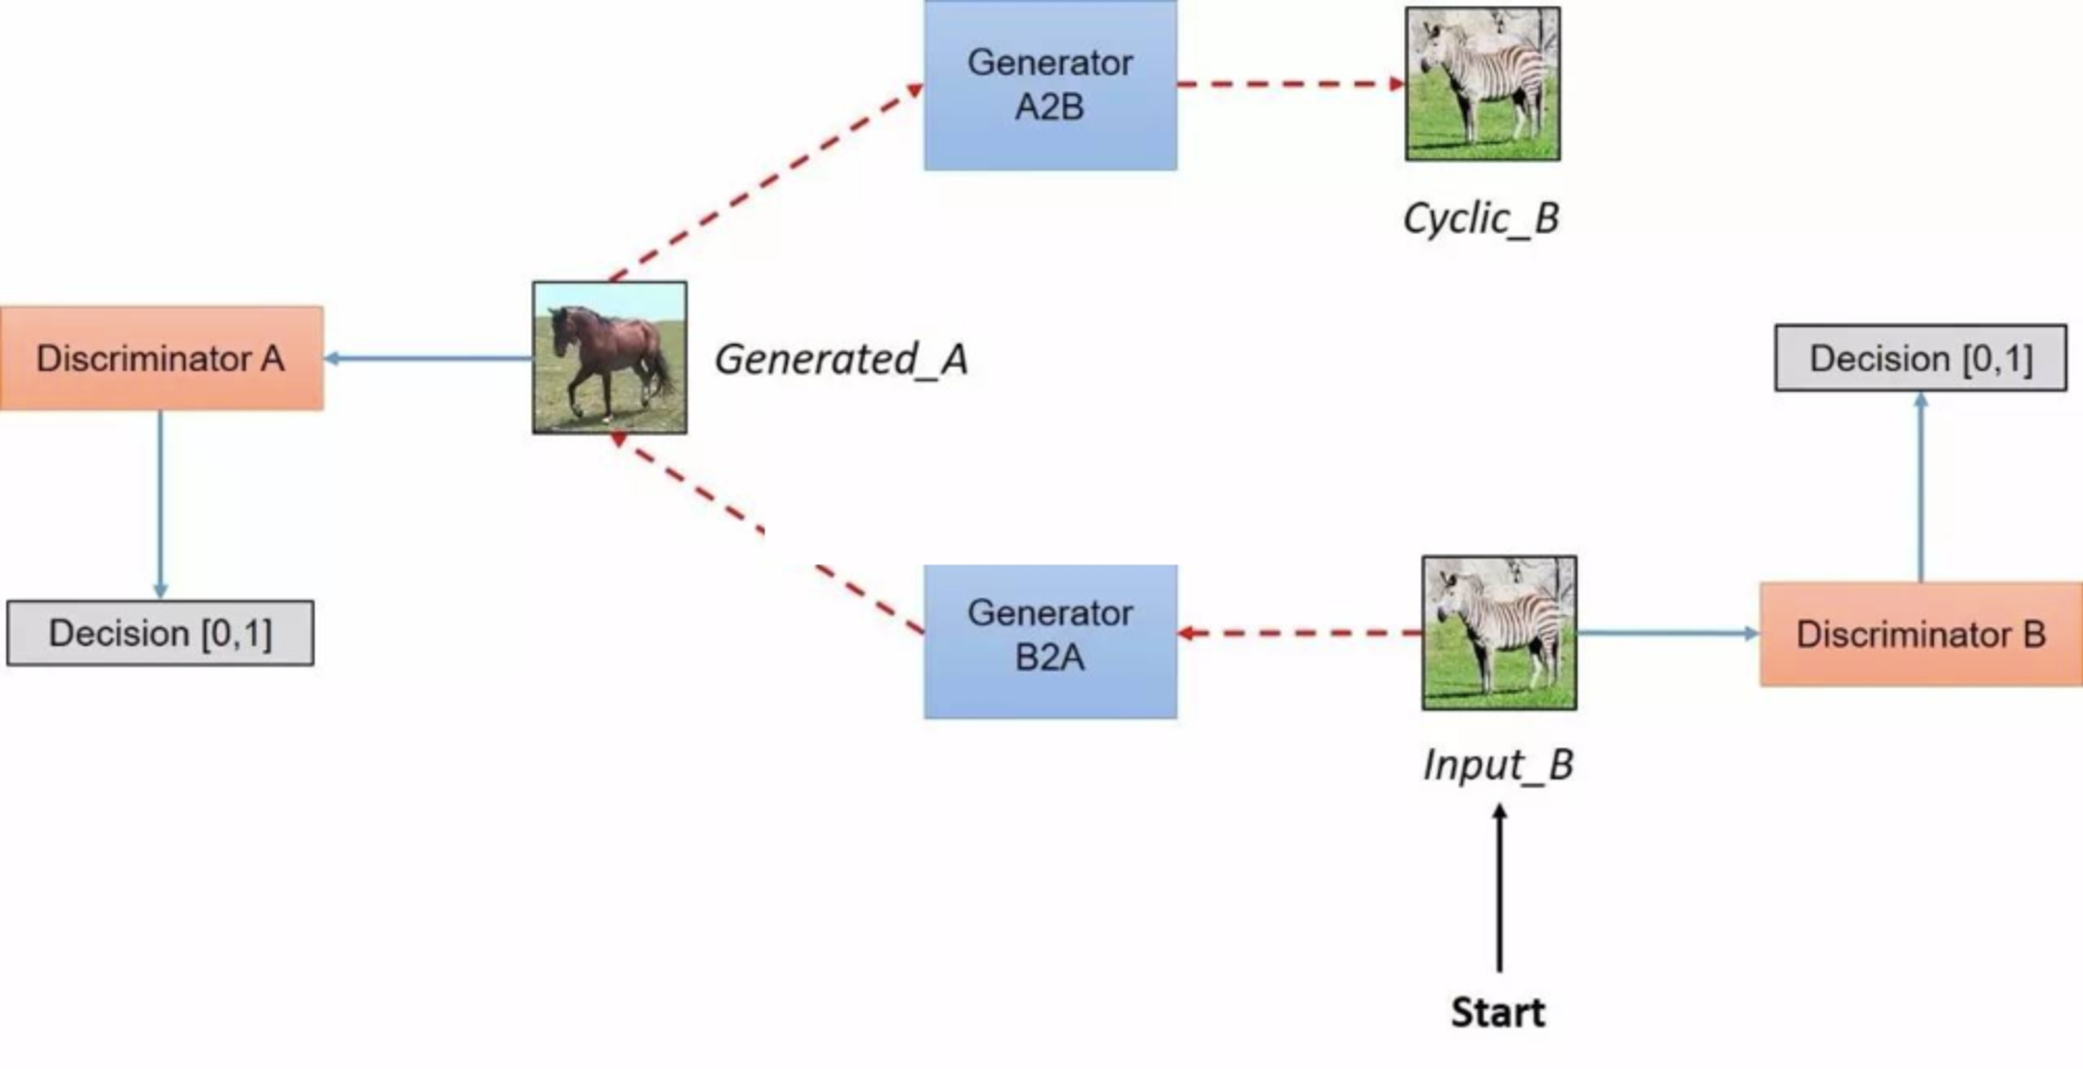
\includegraphics[width=0.45\textwidth]{images/agr.pdf}
\end{minipage}}
\subfigure[b]{
  \begin{minipage}[b]{0.9\textwidth}
  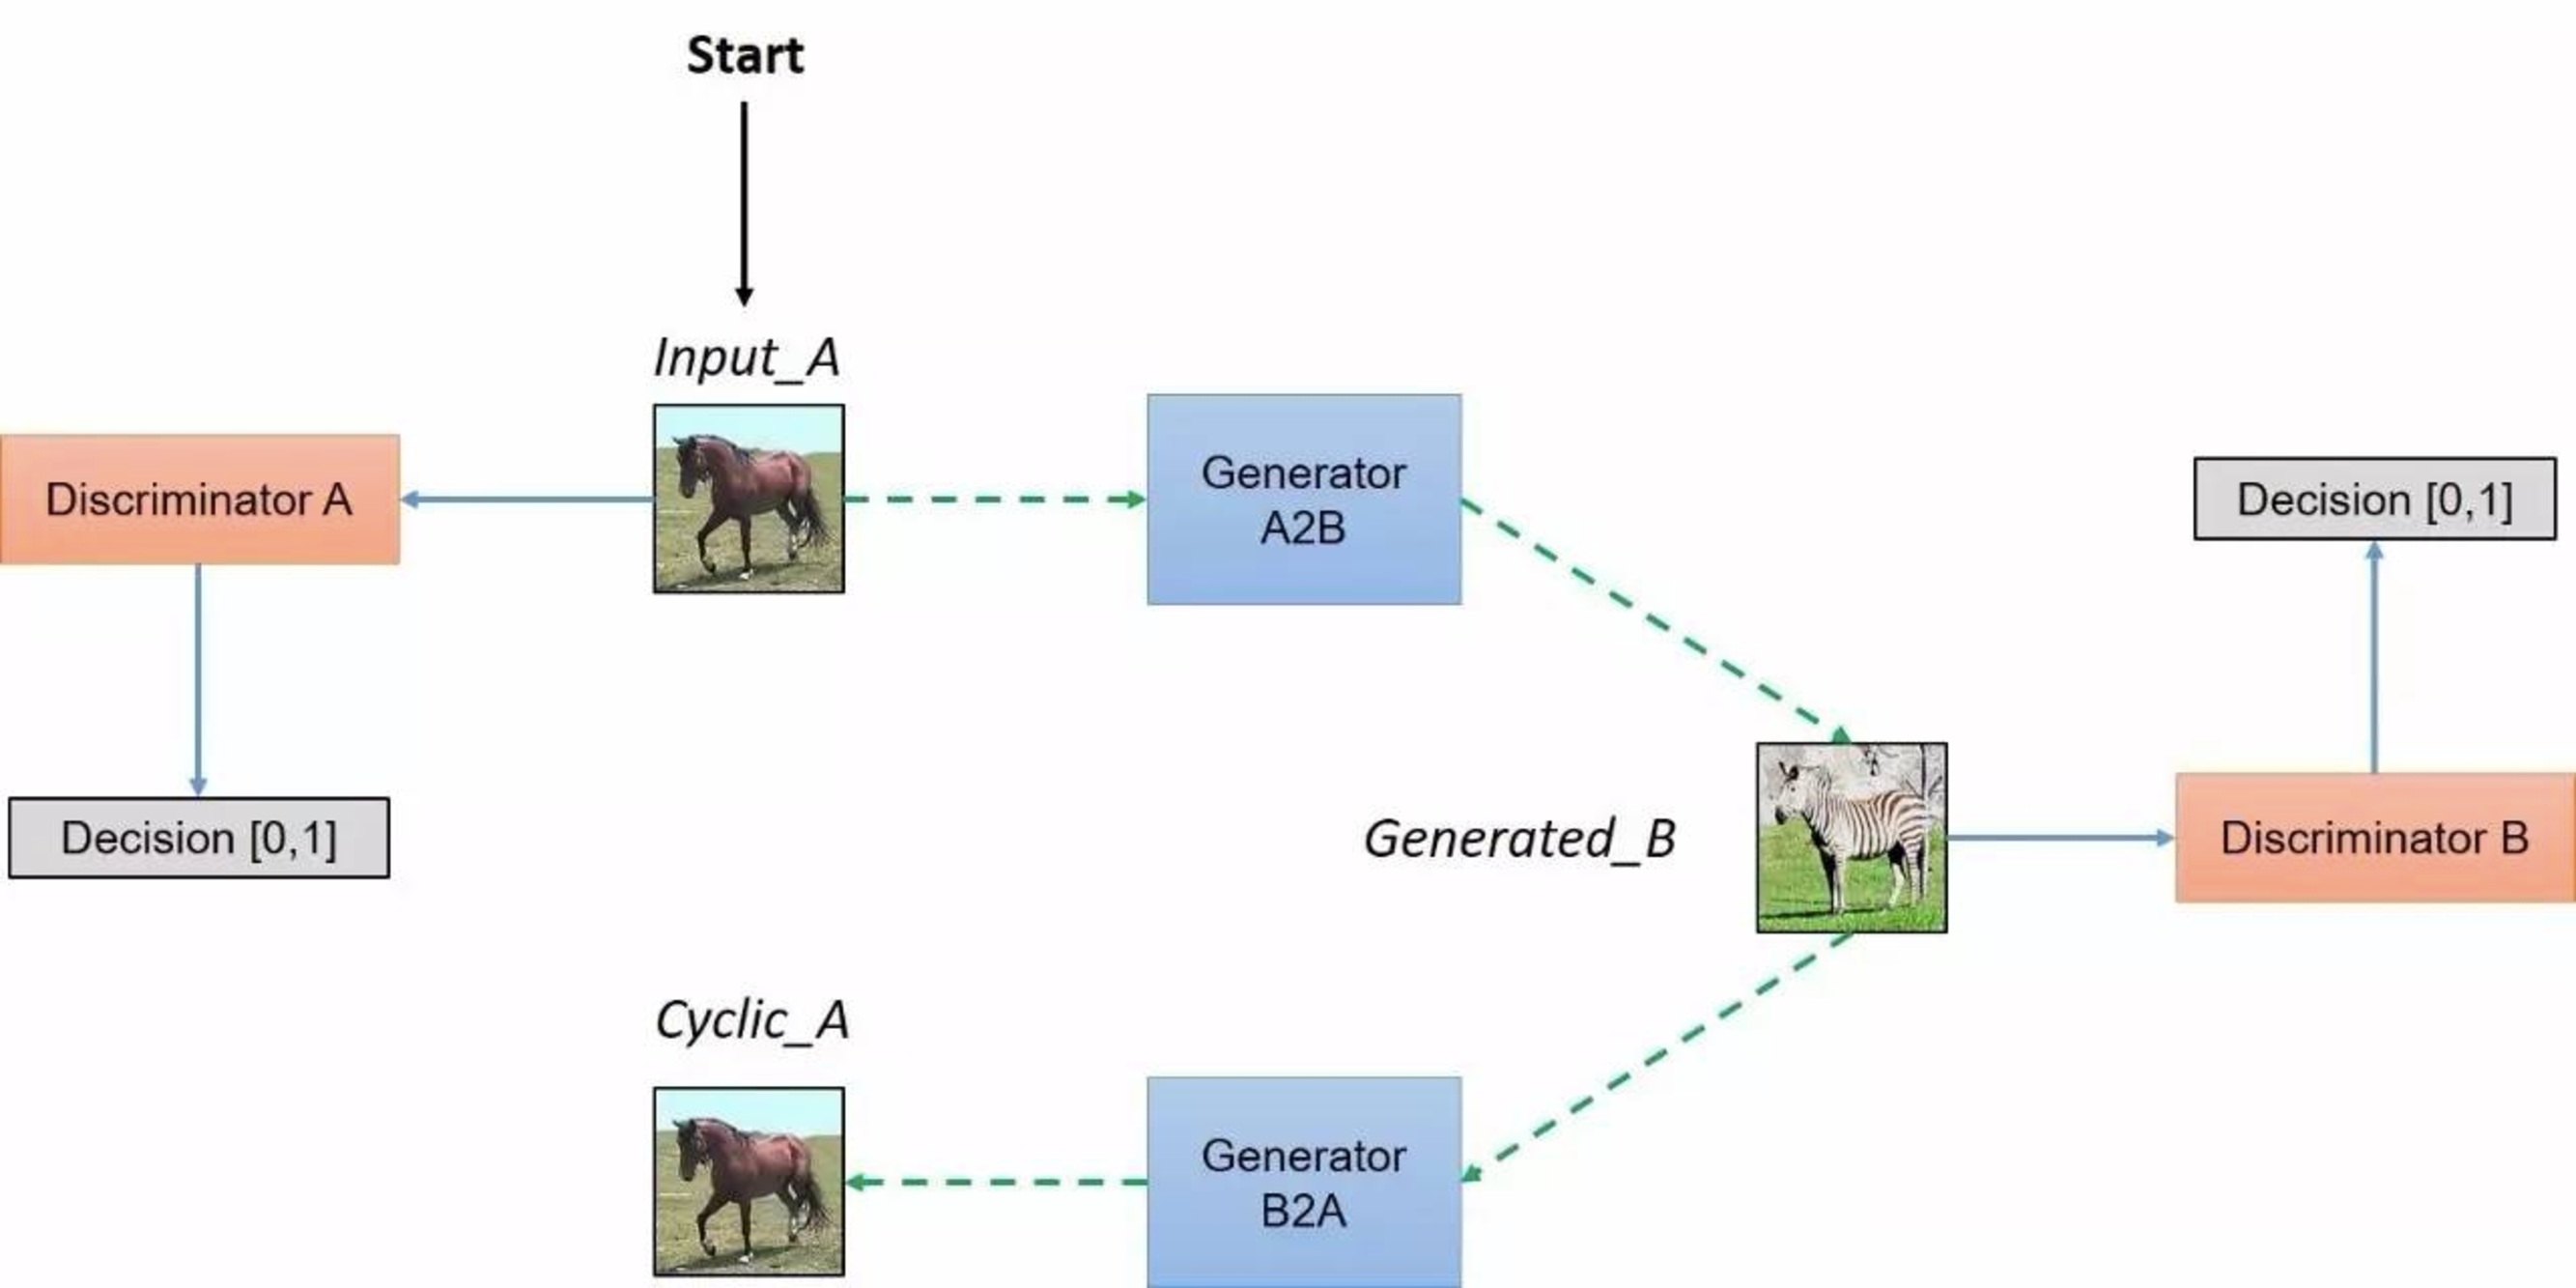
\includegraphics[width=0.45\textwidth]{images/agr1.pdf}
\end{minipage}} 
\caption{The model acquires an input image from the domain DA, 
which is passed to the first generator GeneratorA→B, 
whose task is to convert a given image from the 
domain DA to an image in the target domain DB. 
This newly generated image is then passed to another generator, 
GeneratorB→A, whose task is to convert back to 
the image CyclicA in the original domain DA,
which can be compared to the autoencoder. 
This output image must be similar to the 
original input image and is used to define 
meaningful mappings that did not exist in the unpaired data set.} 
\label{fig:1}
\end{figure}

%-------------------------------------------------------------------------
\subsection{Algorithm flow}

\begin{algorithm}
	\caption{k, is a hyperparameter.We used k = 1, the least expensive option, in our experiments}
    \label{alg}
	\begin{algorithmic}[1]
	\REQUIRE  Image A dataset  $\mathbf{R}$,  Image B dataset  $\mathbf{X}$, number of iterations n 
    \FOR{$i = 1$ to $n$}
      \STATE\FOR{$i = 1$ to $k$}
      \STATE Sample minibatch of m noise Samples from noise prior Pg(z)
      \STATE Sample minibatch of n examples from data generationg districution Pdata(x)
      \STATE Update the discriminator by ascending its stochastic gradient:
      \STATE \begin{align}
        \bigtriangledown_{\theta_{d}} 1/M \sum_{n=1}^M [\log D(x^{i}) + \log (1-D(G(z^{i})))]
      \end{align}
      \STATE\ENDFOR
      \STATE Sample minibatch of m noise Samples from noise prior Pg(z)
      \STATE Update the discriminator by decending its stochastic gradient:
      \STATE \begin{align}
        \bigtriangledown_{\theta_{g}} 1/M \sum_{n=1}^M \log (1-D(G(z^{i})))
      \end{align}
    \ENDFOR
	\end{algorithmic}
\end{algorithm}


\subsection{ Experimental data set}
The source of the experimental data set is the data set provided by the original author, 
the source of the data set:\url{https://people.eecs.berkeley.edu/~taesung_park/CycleGAN/datasets/}

\subsection{Experimental result}
The experimental results are as shown picture\ref{fig:loss200_02}\ref{fig:change}

\begin{figure}
  \centering
    \subfigure{
      \includegraphics[width=0.46\textwidth]{images/loss200_02.pdf}}
  \caption{
  As the epoch continues to increase,
  the accuracy of GA and GB 
  keep rising and gradually stabilizes.
  the stable values of $D_A$ is about 0.83,
  the stable values of $D_B$ is about 0.76.}
  \label{fig:loss200_02}
\end{figure}


\begin{figure}
  \centering
    \subfigure{
      \label{s}
      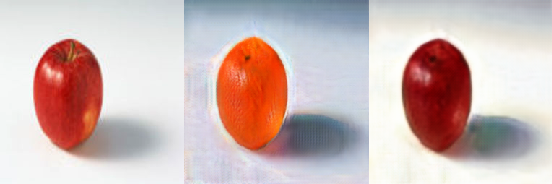
\includegraphics[width=0.46\textwidth]{images/Test_result_164.png}}
      \space \space \space \space \space \space \space
     \subfigure{
      \label{}
      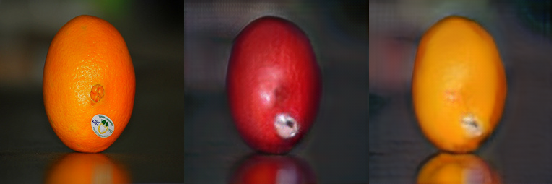
\includegraphics[width=0.46\textwidth]{images/Test_result_235.png}}
       \subfigure{
      \label{}
      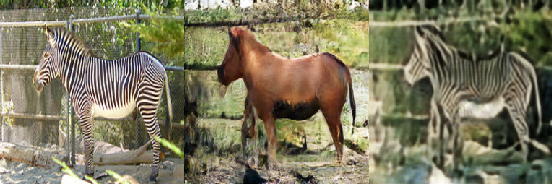
\includegraphics[width=0.46\textwidth]{images/Test_result_86.png}}
       \subfigure{
      \label{}
      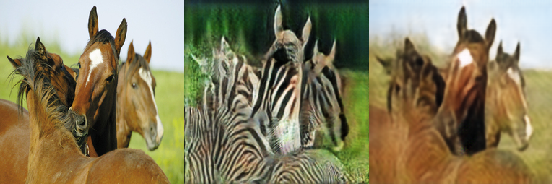
\includegraphics[width=0.46\textwidth]{images/Test_result_2.png}}
  \caption{Basically, the conversion between unpaired images and images has been implemented, but the conversion effect is not very good, and the converted image is not smooth enough. In the pixel processing, our model still needs improvement.
  }
  
  \label{fig:change}
  
  \end{figure}

\subsection{Performance comparison of different image migration algorithms}
As shown in the table\ref{table:performance}, 
Cyclegan basically realizes the conversion 
between unpaired pictures, 
but the image conversion effect is slightly 
worse than other image migration algorithms. 
The results obtained from the experiment do 
not affect the intuitive judgment of the human eye.

\begin{table}
  \center
  \caption{}
  \label{table:performance}
  \resizebox{0.46\textwidth}{!}{
  \begin{tabular}{|c|c|c|c|c|c|c|c|c|}
  \hline
   &\multicolumn{1}{|c|}{Map to Photo}& \multicolumn{1}{|c|}{Photo to  Map}\\
  \hline
   & Error rate  &  Error rate\\
  \hline
  CoGAN\cite{CoGAN} & 1.1\% & 1.4\% \\
  SimGAN\cite{SimGAN} &1.6\% & 2.8\% \\
  CycleGAN(our) & 23.6\% &22.4\% \\
  
  \hline
  \end{tabular}
  }
  \end{table}
  
  \subsection{Effect of algorithm parameters}
  When obtaining the optimal parameters of the model,
 we use the small epoch to continuously test the optimal parameters of the approximation model. 
 Finally, the learning rate is best around 0.002.

\begin{figure}
  \centering
    \subfigure{
      \label{subfig:loss200_02}
      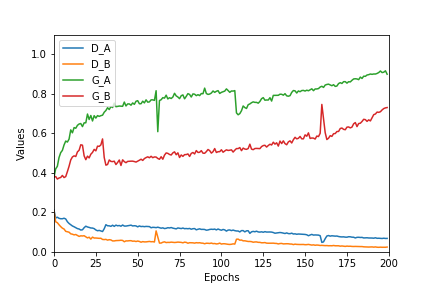
\includegraphics[width=0.46\textwidth]{images/loss_200_02.png}}
      \space \space \space \space \space \space \space
     \subfigure{
      \label{subfig:loss20_02}
      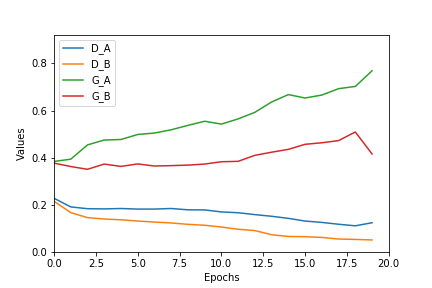
\includegraphics[width=0.46\textwidth]{images/loss_20_02.png}}
  \caption{The epoch value increases and 
  the value increases when the 
  accuracy reaches stability.}
  \label{fig:loss_200_20}
  
  \centering
    
     \subfigure{
      \label{subfig:loss20_015}
      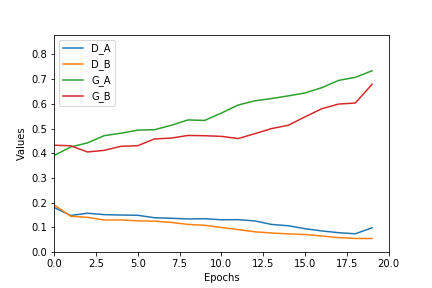
\includegraphics[width=0.46\textwidth]{images/loss_20_015.png}}
      \subfigure{
      \label{subfig:loss20_030}
      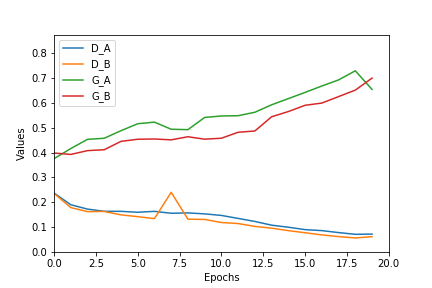
\includegraphics[width=0.46\textwidth]{images/loss_20_030.png}}
  \caption{When the learning rate is equal to 0.003, there is an over-fitting phenomenon. When the learning rate is 0.0015, the image is slightly worse than the learning rate of 0.002.}
  \label{fig:loss_02_015_030}
  
\end{figure}




%------------------------------------------------------------------------
\section{conclusion }

In this report, we implement the code of 
“Unpaired Image-to-Image Translation 
using Cycle-Consistent Adversarial Networks”. 
The success of our cyclegan model is 
due to the standing of the work of our predecessors.
This recurring experiment gives us a deeper 
understanding of GAN and encourages us to focus on our deep learning.



\section{Code Implementation }

Code implementation is a fine-tuning, referring \href{https://github.com/eriklindernoren/PyTorch-GAN}{PyTorch-GAN}
and 
\href{https://github.com/junyanz/pytorch-CycleGAN-and-pix2pix}{pytorch-CycleGAN-and-pix2pix}






\inputpython{11.py}{1}{25}


Since some code lines are too long, the cvpr template cannot display the code properly. The code item address is given below.	\url{https://github.com/zfr0411/CycleGAN}




{\small
\bibliographystyle{ieee_fullname}
\bibliography{egbib}
}








\end{document}
